\documentclass[14pt]{minimal}
\usepackage{tikz}
\usetikzlibrary{backgrounds}
\usetikzlibrary{matrix}
\usetikzlibrary{positioning}
\usetikzlibrary{tikzmark}

\begin{document}
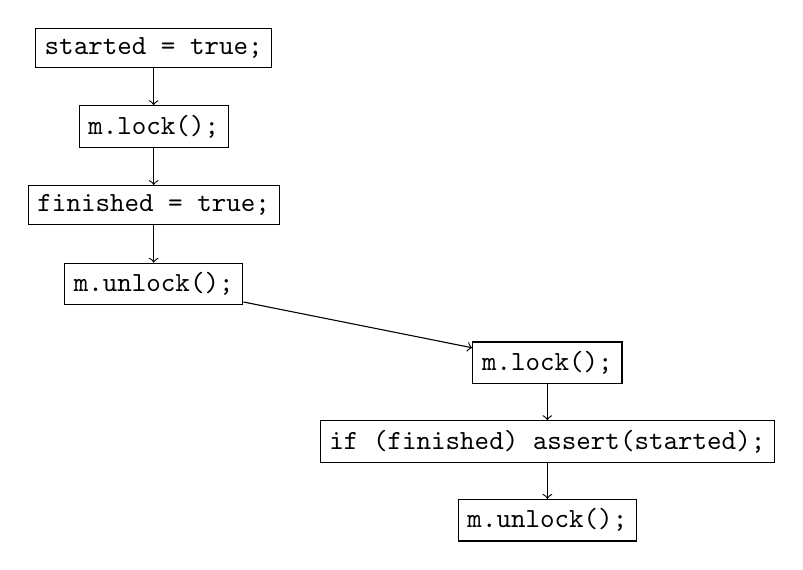
\begin{tikzpicture}[every node/.style={draw,solid,color=black}]
\node(t1a) at (0, 0) {\texttt{started = true;}};
\node(t1b) at (0, -1) {\texttt{m.lock();}};
\node(t1c) at (0, -2) {\texttt{finished = true;}};
\node(t1d) at (0, -3) {\texttt{m.unlock();}};

\node(t2a) at (5, -4) {\texttt{m.lock();}};
\node(t2b) at (5, -5) {\texttt{if (finished) assert(started);}};
\node(t2c) at (5, -6) {\texttt{m.unlock();}};

\draw[->] (t1a)--(t1b); \draw[->] (t1b)--(t1c); \draw[->] (t1c)--(t1d);
\draw[->] (t2a)--(t2b); \draw[->] (t2b)--(t2c);
\draw[->] (t1d)--(t2a);
\end{tikzpicture}

\clearpage
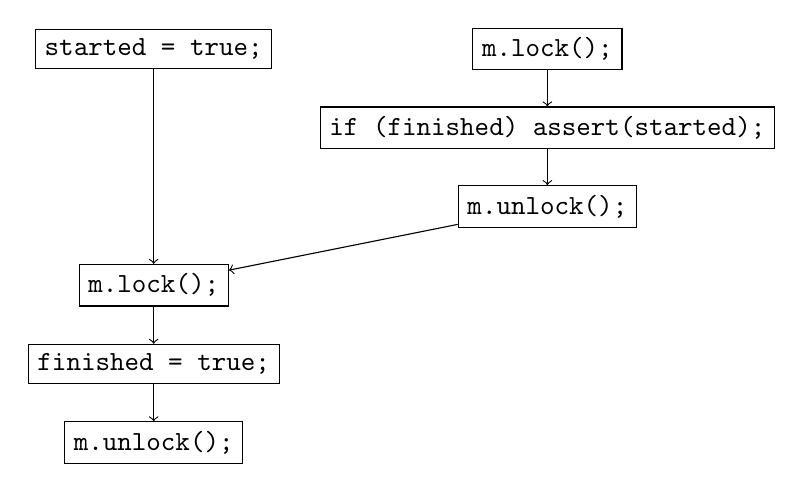
\begin{tikzpicture}[every node/.style={draw,solid,color=black}]
\node(t1a) at (0, 0) {\texttt{started = true;}};
\node(t1b) at (0, -3) {\texttt{m.lock();}};
\node(t1c) at (0, -4) {\texttt{finished = true;}};
\node(t1d) at (0, -5) {\texttt{m.unlock();}};

\node(t2a) at (5, 0) {\texttt{m.lock();}};
\node(t2b) at (5, -1) {\texttt{if (finished) assert(started);}};
\node(t2c) at (5, -2) {\texttt{m.unlock();}};

\draw[->] (t1a)--(t1b); \draw[->] (t1b)--(t1c); \draw[->] (t1c)--(t1d);
\draw[->] (t2a)--(t2b); \draw[->] (t2b)--(t2c);
\draw[->] (t2c)--(t1b);
\end{tikzpicture}

\clearpage
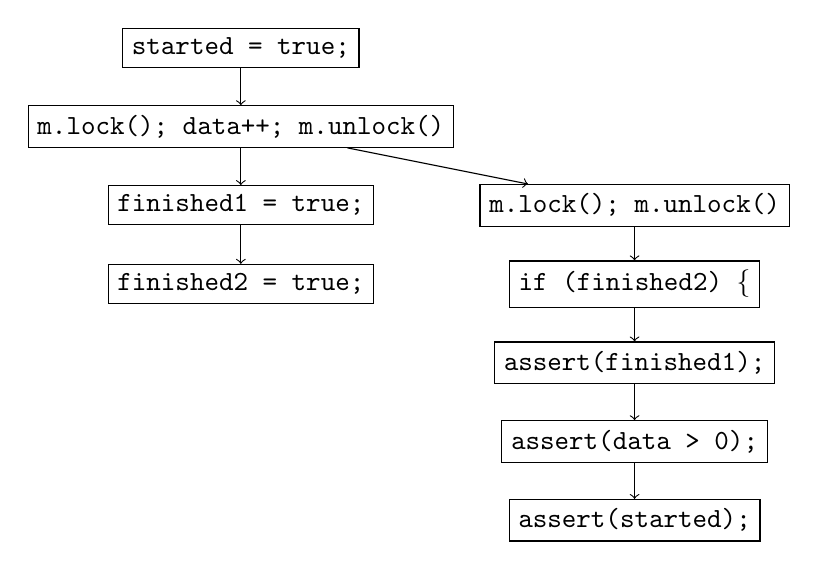
\begin{tikzpicture}[every node/.style={draw,solid,color=black}]
\node(t1a) at (0, 0) {\texttt{started = true;}};
\node(t1b) at (0, -1) {\texttt{m.lock(); data++; m.unlock()}};
\node(t1c) at (0, -2) {\texttt{finished1 = true;}};
\node(t1d) at (0, -3) {\texttt{finished2 = true;}};

\node(t2a) at (5, -2) {\texttt{m.lock(); m.unlock()}};
\node(t2b) at (5, -3) {\texttt{if (finished2) \{}};
\node(t2c) at (5, -4) {\texttt{assert(finished1);}};
\node(t2d) at (5, -5) {\texttt{assert(data > 0);}};
\node(t2e) at (5, -6) {\texttt{assert(started);}};

\draw[->] (t1a)--(t1b); \draw[->] (t1b)--(t1c); \draw[->] (t1c)--(t1d);
\draw[->] (t2a)--(t2b); \draw[->] (t2b)--(t2c); \draw[->] (t2c)--(t2d); \draw[->] (t2d)--(t2e);
\draw[->] (t1b)--(t2a);
\end{tikzpicture}

\clearpage
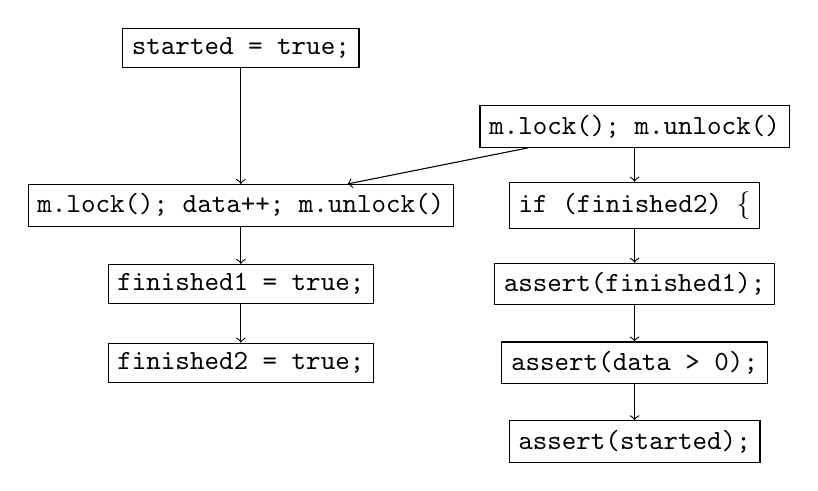
\begin{tikzpicture}[every node/.style={draw,solid,color=black}]
\node(t1a) at (0, 0) {\texttt{started = true;}};
\node(t1b) at (0, -2) {\texttt{m.lock(); data++; m.unlock()}};
\node(t1c) at (0, -3) {\texttt{finished1 = true;}};
\node(t1d) at (0, -4) {\texttt{finished2 = true;}};

\node(t2a) at (5, -1) {\texttt{m.lock(); m.unlock()}};
\node(t2b) at (5, -2) {\texttt{if (finished2) \{}};
\node(t2c) at (5, -3) {\texttt{assert(finished1);}};
\node(t2d) at (5, -4) {\texttt{assert(data > 0);}};
\node(t2e) at (5, -5) {\texttt{assert(started);}};

\draw[->] (t1a)--(t1b); \draw[->] (t1b)--(t1c); \draw[->] (t1c)--(t1d);
\draw[->] (t2a)--(t2b); \draw[->] (t2b)--(t2c); \draw[->] (t2c)--(t2d); \draw[->] (t2d)--(t2e);
\draw[->] (t2a)--(t1b);
\end{tikzpicture}
\end{document}
